\documentclass[letter,11pt]{article}

\usepackage[spanish,es-nodecimaldot]{babel}
\usepackage[utf8]{inputenc}

\usepackage{lmodern}
\usepackage[T1]{fontenc}
\usepackage{textcomp}

\usepackage{framed}
\usepackage[svgnames]{xcolor}
\colorlet{shadecolor}{Gainsboro!50}

\usepackage{enumitem}
\usepackage{graphicx}
\usepackage{pstricks}

\usepackage{anysize}
\marginsize{3cm}{2cm}{2cm}{3cm}

\usepackage{siunitx}
\usepackage{amsmath}
\usepackage{array}
\usepackage{alltt}

\usepackage{fancyhdr}
\usepackage{lastpage}
\pagestyle{fancy}
\fancyhf{}
\fancyhead[LE,RO]{Física Básica II}
\fancyfoot[CO,CE]{\thepage\ de \pageref{LastPage}}

\special{papersize=215.9mm,279.4mm}

\usepackage[
    pdfauthor={Carlos Eduardo Caballero Burgoa},%
    pdftitle={Física Básica II},%
    pdfsubject={Tarea 7},%
    colorlinks,%
    citecolor=black,%
    filecolor=black,%
    linkcolor=black,%
    urlcolor=black,
    breaklinks]{hyperref}
\usepackage{breakurl}

\newcommand{\blankpage}{
\newpage
\thispagestyle{empty}
\mbox{}
\newpage
}

\renewcommand{\arraystretch}{1.2}

\begin{document}

\begin{center}
    {\Large \bf{\underline{Tarea \#7}}}
\end{center}

Calcular el centro de masa del siguiente sistema compuesto. La barra delgada
tiene densidad lineal uniforme y longitud igual a $2 [m]$.

\begin{figure}[!h]
\centering
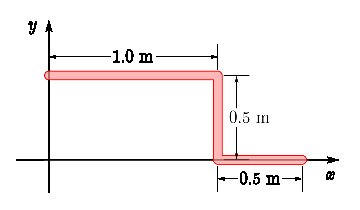
\includegraphics[scale=1.25]{resources/f1.eps}
\end{figure}

\vspace{0.5cm}
\textbf{\underline{Solución}:} \\

Se calculará el centro de masa, separando la barra en tres componentes y sumando
los centros de masa respectivos.

\begin{equation}
    \vec{r}_{cm} = \frac{1}{M} \sum_{i=1}^{N} \vec{r_i} \cdot m_i
\label{base}
\tag{centro de masa}
\end{equation}

\vspace{0.5cm}
De resultados anteriores conocemos el centro de masa de una barra horizontal con
origen en un extremo de la misma, además de una barra vertical:

\begin{equation}
    \vec{r}_{cm} = \frac{L}{2} \hat{i}
\label{horizontal}
\tag{barra horizontal}
\end{equation}

\begin{equation}
    \vec{r}_{cm} = \frac{L}{2} \hat{j}
\label{horizontal}
\tag{barra vertical}
\end{equation}

\vspace{0.5cm}
Sabiendo que la densidad es uniforme entonces:

\begin{equation*}
    M = m_1 + m_2 + m_3 = 2m + m + m = 4m
\end{equation*}

\vspace{0.5cm}
Por tanto:

\begin{equation*}
    \vec{r}_{cm} = \frac{1}{M} (\vec{r}_1 \cdot m_1 + \vec{r}_2 \cdot m_2 + \vec{r}_3 \cdot m_3)
\end{equation*}
\begin{equation*}
    \vec{r}_{cm} = \frac{1}{4m} (\vec{r}_1 \cdot m_1 + \vec{r}_2 \cdot m_2 + \vec{r}_3 \cdot m_3)
\end{equation*}
\begin{equation*}
    \vec{r}_{cm} = \frac{1}{4m} \left[ \left(\frac{1}{2} \hat{i} + \frac{1}{2} \hat{j}\right) \cdot 2m + \left(\hat{i}+\frac{1}{4} \hat{j}\right) \cdot m + \left(\frac{5}{4} \hat{i}\right) \cdot m \right]
\end{equation*}

\vspace{0.5cm}
Separando en sus componentes, obtenemos:

\begin{equation*}
    x_{cm} = \frac{1}{4m} \cdot \left(m + m + \frac{5m}{4}\right) = \frac{1}{4m} \cdot \frac{13m}{4} = \frac{13}{16} = 0.8125 [m]
\end{equation*}
\begin{equation*}
    y_{cm} = \frac{1}{4m} \cdot \left(m + \frac{m}{4} + 0\right) = \frac{1}{4m} \cdot \frac{5m}{4} = \frac{5}{16} = 0.3125 [m]
\end{equation*}

\vspace{0.5cm}
Resultando:

\begin{equation}
    \vec{r}_{cm} = (0.8125 \hat{i} + 0.3125 \hat{j}) [m]
\end{equation}

\end{document}

